% Equivalent of enabling ``-Wall -Wextra'' -- extra compile warnings.
\RequirePackage[l2tabu, orthodox]{nag}

\documentclass[capstoc,capschap,draftcls]{rpisudiss}
\usepackage[utf8]{inputenc} % set input encoding (not needed with XeLaTeX)

\usepackage{url}

\usepackage{graphicx}

% Supports cross-references to labels of form format:name (like fig:mypicture) and formats them nicer
% (Figure X) when you use \prettyref{fig:mypicture} instead of \ref{fig:mypicture}
\usepackage{prettyref}


\begin{document}

\chapter{middle}

A VR~JuggLua application uses both the osgLua module
and the VR~Juggler bindings included in the VR~JuggLua framework
to access a complete set of virtual reality functionality from Lua
(Figure \ref{fig:System-diagram}).
\begin{figure}
    \centering
    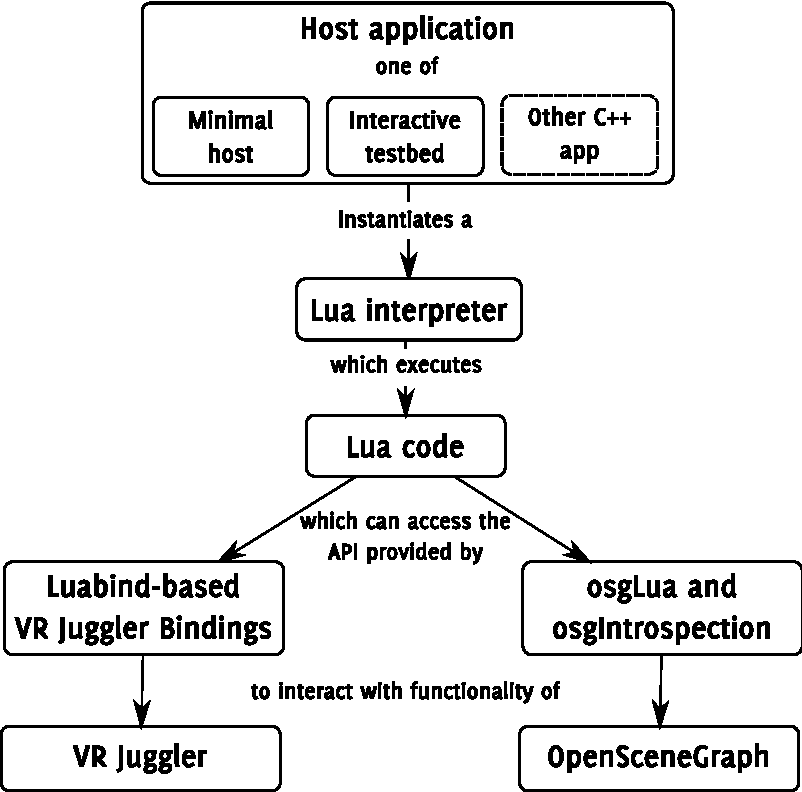
\includegraphics[width=1\columnwidth]{accessdiagram}
    \caption{\label{fig:System-diagram}System diagram}
\end{figure}


\section{Bla bla}
Later development
extended its use from high-end graphics systems to commodity computer
clusters.

frameworks. It has evolved into a commercial solution integrating
clustering support and focusing on multi-screen application development.
VR~Juggler introduced a highly modular architecture for VR applications

\subsection{bla bla bla}
The commercial
VR authoring environment Virtools%
\footnote{\url{http://www.virtools.com/}%
} integrates a custom scripting language, VSL, for content creation.

\end{document}
